\documentclass[runningheads]{llncs}
\usepackage{graphicx}
\usepackage{booktabs}
\usepackage{multirow}
\usepackage{microtype}
\usepackage{amsmath}
\usepackage[T5,T1]{fontenc}
\usepackage{tikz}
\usetikzlibrary{arrows.meta,positioning,fit}
\usepackage[hidelinks]{hyperref}
\emergencystretch=1em
\setlength{\textfloatsep}{7pt plus 1pt minus 2pt}
\setlength{\intextsep}{7pt plus 1pt minus 2pt}
\newcommand{\method}{CEARF-N}
\newcommand{\rr}{\rho}
% Generated by summarize_dynamic_beta.py; do not edit manually.
\newcommand{\DynamicSeedCount}{3}
\newcommand{\DynamicVideoRtwenty}{.14735}
\newcommand{\DynamicVideoBetaMean}{.572}
\newcommand{\DynamicVideoBetaWithinSD}{.013}
\newcommand{\DynamicVideoNetVsGlobal}{15}
\newcommand{\DynamicVideoLowBetaAdv}{-.01026}
\newcommand{\DynamicVideoHighBetaAdv}{.00589}
\newcommand{\DynamicVideoAllocationGap}{.01614}
\newcommand{\DynamicVideoOOFRows}{4000 (0.0)}
\newcommand{\DynamicVideoActionable}{1666 (25.4)}
\newcommand{\DynamicVideoActionableShare}{.4165 (.0063)}
\newcommand{\DynamicVideoGlobalBeta}{.57748 (.00705)}
\newcommand{\DynamicVideoCandidatePool}{94,762}
\newcommand{\DynamicVideoDeclaredValidation}{5,000}
\newcommand{\DynamicVideoTargetsRemoved}{0}
\newcommand{\DynamicVideoDeclaredOOFOverlap}{0}
\newcommand{\DynamicVideoCandidateOOFOverlap}{5,000}
\newcommand{\DynamicVideoEligible}{89,762}
\newcommand{\DynamicVideoProfileHash}{623fdf1e}
\newcommand{\DynamicVideoGateHash}{3df29839}
\newcommand{\DynamicVideoRescues}{4451 (29.9)}
\newcommand{\DynamicVideoDamage}{1766 (43.3)}
\newcommand{\DynamicVideoNetRescues}{2685 (19.1)}
\newcommand{\DynamicVideoPrimaryU}{.11281 (.00021)}
\newcommand{\DynamicVideoContextMLPU}{.11303 (.00026)}
\newcommand{\DynamicVideoFullLinearU}{.11295 (.00032)}
\newcommand{\DynamicVideoFullMLPU}{.11310 (.00044)}
\newcommand{\DynamicVideoNoCrossExpertU}{.11297 (.00034)}
\newcommand{\DynamicVideoNoMemoryCertaintyU}{.11309 (.00026)}
\newcommand{\DynamicVideoKTenU}{.11219 (.00018)}
\newcommand{\DynamicVideoKTwentyU}{.11281 (.00021)}
\newcommand{\DynamicVideoKSixtyU}{.11163 (.00026)}
\newcommand{\DynamicBabyRtwenty}{.05669}
\newcommand{\DynamicBabyBetaMean}{.541}
\newcommand{\DynamicBabyBetaWithinSD}{.005}
\newcommand{\DynamicBabyNetVsGlobal}{-3}
\newcommand{\DynamicBabyLowBetaAdv}{.00245}
\newcommand{\DynamicBabyHighBetaAdv}{.00118}
\newcommand{\DynamicBabyAllocationGap}{-.00127}
\newcommand{\DynamicBabyOOFRows}{4000 (0.0)}
\newcommand{\DynamicBabyActionable}{845 (13.1)}
\newcommand{\DynamicBabyActionableShare}{.2113 (.0033)}
\newcommand{\DynamicBabyGlobalBeta}{.54335 (.00923)}
\newcommand{\DynamicBabyCandidatePool}{150,777}
\newcommand{\DynamicBabyDeclaredValidation}{5,000}
\newcommand{\DynamicBabyTargetsRemoved}{0}
\newcommand{\DynamicBabyDeclaredOOFOverlap}{0}
\newcommand{\DynamicBabyCandidateOOFOverlap}{5,000}
\newcommand{\DynamicBabyEligible}{145,777}
\newcommand{\DynamicBabyProfileHash}{b0fb3c22}
\newcommand{\DynamicBabyGateHash}{3556eb83}
\newcommand{\DynamicBabyRescues}{3889 (111.5)}
\newcommand{\DynamicBabyDamage}{1191 (55.9)}
\newcommand{\DynamicBabyNetRescues}{2698 (55.8)}
\newcommand{\DynamicBabyPrimaryU}{.04343 (.00032)}
\newcommand{\DynamicBabyContextMLPU}{.04345 (.00030)}
\newcommand{\DynamicBabyFullLinearU}{.04349 (.00041)}
\newcommand{\DynamicBabyFullMLPU}{.04348 (.00039)}
\newcommand{\DynamicBabyNoCrossExpertU}{.04345 (.00035)}
\newcommand{\DynamicBabyNoMemoryCertaintyU}{.04347 (.00041)}
\newcommand{\DynamicBabyKTenU}{.04261 (.00034)}
\newcommand{\DynamicBabyKTwentyU}{.04343 (.00032)}
\newcommand{\DynamicBabyKSixtyU}{.04354 (.00027)}
\newcommand{\DynamicDigiRtwenty}{.51701}
\newcommand{\DynamicDigiBetaMean}{.420}
\newcommand{\DynamicDigiBetaWithinSD}{.010}
\newcommand{\DynamicDigiNetVsGlobal}{-1}
\newcommand{\DynamicDigiLowBetaAdv}{-.01263}
\newcommand{\DynamicDigiHighBetaAdv}{-.01541}
\newcommand{\DynamicDigiAllocationGap}{-.00278}
\newcommand{\DynamicDigiOOFRows}{4000 (0.0)}
\newcommand{\DynamicDigiActionable}{3298 (8.2)}
\newcommand{\DynamicDigiActionableShare}{.8245 (.0020)}
\newcommand{\DynamicDigiGlobalBeta}{.41848 (.00284)}
\newcommand{\DynamicDigiCandidatePool}{133,724}
\newcommand{\DynamicDigiDeclaredValidation}{5,000}
\newcommand{\DynamicDigiTargetsRemoved}{5,000}
\newcommand{\DynamicDigiDeclaredOOFOverlap}{0}
\newcommand{\DynamicDigiCandidateOOFOverlap}{5,000}
\newcommand{\DynamicDigiEligible}{128,724}
\newcommand{\DynamicDigiProfileHash}{c0f021cd}
\newcommand{\DynamicDigiGateHash}{13a5b5af}
\newcommand{\DynamicDigiRescues}{3076 (55.8)}
\newcommand{\DynamicDigiDamage}{1693 (43.1)}
\newcommand{\DynamicDigiNetRescues}{1383 (86.6)}
\newcommand{\DynamicDigiPrimaryU}{.41332 (.00115)}
\newcommand{\DynamicDigiContextMLPU}{.41331 (.00108)}
\newcommand{\DynamicDigiFullLinearU}{.41345 (.00094)}
\newcommand{\DynamicDigiFullMLPU}{.41321 (.00105)}
\newcommand{\DynamicDigiNoCrossExpertU}{.41304 (.00093)}
\newcommand{\DynamicDigiNoMemoryCertaintyU}{.41357 (.00079)}
\newcommand{\DynamicDigiKTenU}{.41271 (.00081)}
\newcommand{\DynamicDigiKTwentyU}{.41332 (.00115)}
\newcommand{\DynamicDigiKSixtyU}{.41227 (.00074)}

% Generated by benchmark_dynamic_beta_inference.py; do not edit.
\newcommand{\DynamicRuntimeVideoQueries}{94,762}
\newcommand{\DynamicRuntimeVideoGateUs}{1.171}
\newcommand{\DynamicRuntimeVideoPostUs}{85.89}
\newcommand{\DynamicRuntimeVideoExpertMs}{3.710}
\newcommand{\DynamicRuntimeVideoTotalMs}{3.796}
\newcommand{\DynamicRuntimeBabyQueries}{150,777}
\newcommand{\DynamicRuntimeBabyGateUs}{1.184}
\newcommand{\DynamicRuntimeBabyPostUs}{87.57}
\newcommand{\DynamicRuntimeBabyExpertMs}{4.031}
\newcommand{\DynamicRuntimeBabyTotalMs}{4.119}
\newcommand{\DynamicRuntimeDigiQueries}{60,858}
\newcommand{\DynamicRuntimeDigiGateUs}{.774}
\newcommand{\DynamicRuntimeDigiPostUs}{80.60}
\newcommand{\DynamicRuntimeDigiExpertMs}{2.428}
\newcommand{\DynamicRuntimeDigiTotalMs}{2.509}
\newcommand{\DynamicRuntimeMaxBetaError}{$5.96\times10^{-8}$}
\newcommand{\DynamicRuntimeExactTopTwenty}{exact}


\begin{document}
\title{\method{}: Bounded Out-of-Fit Dynamic Rank Allocation for Sparse
Next-Item Recommendation}
\titlerunning{Bounded Out-of-Fit Dynamic Rank Allocation}
\author{Pham Quoc Cuong\inst{1,2} \and
Nguyen Ngoc Minh\inst{1,2} \and
Le Quang Minh\inst{1,2} \and
Nguyen Hoai Nguyet An\inst{1,2}}
\authorrunning{P. Q. Cuong et al.}
\institute{University of Information Technology, Ho Chi Minh City, Vietnam
\and Vietnam National University Ho Chi Minh City, Vietnam\\
\email{\{cuongpq.20,minhnn.20,minhlq.20,annhv.20\}@grad.uit.edu.vn}}
\maketitle

\begin{abstract}
Explicit memory and neural rankers fail on different next-item queries, while
rank-level hybrids commonly assign every query one global fusion weight. We
introduce \method{} (\emph{Contextual Expert-Allocation Rank Fusion with a
Neural residual}).
It is a constrained post-hoc conditional allocator over frozen rankers:
a global prior and bounded query correction are learned continuously from
source-disjoint out-of-fit training ranks. A four-parameter gate predicts
$\beta_q=\beta_{\mathrm{OOF}}+\Delta_{\rm eff}
\tanh(\mathbf w^\top\mathbf z_q+b)$,
$\Delta_{\rm eff}\leq.10$, from three standardized, target-free inference
features. No validation/test label fits or selects a mixing weight.
Its expert interface is rank-only, making it invariant to strictly monotone
score transforms, and it has a closed-form pair-intervention bound.
Full-catalogue, three-seed experiments on two Amazon domains and Diginetica
show that equal/dynamic fusion improves R@20 by 4.6--17.2\% over the stronger
constituent, confirming expert complementarity. The dynamic-specific finding
is narrower: against the training-only global policy, dynamic allocation has
interval-above-zero early-rank gains on Video, while Baby and Diginetica shifts
are undetectable. A fixed same-$\beta$-multiset reassignment is worse on Video
nDCG@20.
\keywords{next-item recommendation \and dynamic rank fusion \and
bounded rank allocation \and sparse recommendation}
\end{abstract}

\section{Introduction}
Modern next-item models strengthen learned representations through recurrent,
state-space, semantic, and mixture-of-experts designs
\cite{li2025survey,sigma2025,hm2rec2026,llm2rec2025,hidlongtail2026}. Sparse
catalogues expose their complement: a rare item may receive few gradient
updates while an observed transition or near-duplicate session remains
decisive. Explicit memory cannot generalize beyond observed edges and overlap.
The practical question is therefore how much each query should trust
heterogeneous evidence.

A global fusion coefficient assigns every query the same trust. A flexible
router adds another estimation surface; separately, benchmark shortcuts and
weak tuning can inflate apparent progress
\cite{shortcut2026,standards2026}. We
instead learn a continuous global prior from out-of-fit training ranks and
permit only a bounded query correction. \method{} pairs PASGR, a compact
semantic GRU, with a memory expert selected from a declared transition,
neighbour-session, and popularity family; the training-only lock selects
neighbour-session memory in every reported domain. The pair is combined by
weighted reciprocal-rank fusion \cite{cormack2009rrf}. Validation may audit
the frozen allocator, and an upstream study had already frozen PASGR, but
neither role fits or selects $\beta$. The proposed object is constrained
post-hoc conditional stacking over frozen rankers, not a new sequence encoder:
rank-space removes raw-score scale, source-disjoint OOF fitting avoids expert
self-fit targets, and a residual bound limits every query-wise intervention.

We ask how much gain is endpoint complementarity versus learned allocation
(RQ1), whether a bounded residual adds conditional value beyond OOF-global
allocation (RQ2), how robust it is to capacity/operator changes (RQ3), and
what inference cost it adds (RQ4).

Our contributions are:
\begin{enumerate}
\item a continuous training-only objective that learns both a global fusion
prior and a bounded per-query correction from reciprocal-rank pairwise
evidence, without enumerating $\beta$;
\item a fully specified rank-interface allocator with five optimized coefficients---one
OOF global logit plus a four-parameter residual gate using only context length,
last-item frequency, and a tail indicator;
\item a three-level attribution protocol separating endpoint complementarity,
OOF-global allocation, and query assignment, with capacity and operator
controls; and
\item a serving audit decomposing feature+gate, rank-fusion, and expert
retrieval latency.
\end{enumerate}
The claim is not that routing always wins, but that a small auditable
controller recovers a reproducible early-rank allocation signal on Video.

\section{Related Work}
\textbf{Experts and fusion.}
Recent session recommenders use state-space recurrence, MoE routing, semantic
initialization, and long-tail constraints
\cite{sigma2025,hm2rec2026,llm2rec2025,hidlongtail2026}. V-SKNN/STAN retrieve
related sessions \cite{ludewig2018vsknn,garg2019stan}; NARM is an attentive
recurrent reference \cite{li2017narm}. RRF combines incommensurate score
spaces through ranks \cite{cormack2009rrf}. The primitive is established; our
contribution is an OOF-trained rank prior plus a raw-score-free residual with
target-free inference features, frozen experts, and an explicit intervention
bound.

\textbf{Conditional allocation and evaluation.}
Neural MoE recommenders route jointly trained representations
\cite{hm2rec2026}; multi-channel retrieval can learn query-dependent ranking
over channel signals \cite{multichannelltr2026}. We instead study a five-scalar
bounded composition over frozen explicit and neural rankers. Because
shortcut-solvable benchmarks and weak offline protocols can inflate progress
\cite{shortcut2026,standards2026}, we report tuned transition/V-SKNN/STAN
baselines, both fusion endpoints, matched-query intervals, operator controls,
and semantic-teacher provenance. A held-out validation gate would consume
validation as meta-training; our source-disjoint OOF fitting keeps declared
validation labels out of allocation. The stacking lineage is detailed in the
supplement.

\section{\method{}}
\subsection{Expert interface: memory and neural ranks}
For query $q=(i_1,\ldots,i_L)$, the memory expert exposes three top-120 candidate
memories: distance/recency-weighted four-step transitions, IDF/recency-weighted
neighbour sessions, and global popularity. Six fixed rank-weight profiles are
evaluated on a disjoint training-only lock subset. The realized primary profile
is session-only, $(0,1,0)$, in every domain and length regime; consequently its
agreement bonus is inactive, while transition and popularity remain controls.

The selected profile first produces one memory ordering $\pi_M$.
Equation~\ref{eq:evidence} is then applied afresh to $\pi_M$ and the neural
ordering $\pi_N$, so the final expert evidences lie in $[0,1]$. If ordering
$e$ assigns rank $r_e(x)$ to item $x$, its evidence is
\begin{equation}
\rr_e(x)=\frac{k+1}{k+r_e(x)},\qquad k=20,
\label{eq:evidence}
\end{equation}
with zero evidence when $x$ is absent. PASGR supplies a separate neural
top-120 list; in our locked cells it is a semantic GRU selected from the
\emph{Prototype-Aligned Semantic Graph Retrieval} candidate family. It encodes
the prefix and scores the full catalogue by normalized state--item dot product.
Its cached semantic teacher is documented as E5-small on Video \cite{wang2022e5}
and TF--IDF/SVD otherwise; the frozen upstream cell is detailed in the
supplement. Prototype transport is off in all three locked cells.

\subsection{Continuous query-conditioned allocation}
Let $\rr_M$ and $\rr_N$ denote the selected memory and neural evidence. The
final score is
\begin{equation}
F_q(x)=(1-\beta_q)\rr_M(x)+\beta_q\rr_N(x).
\label{eq:fusion}
\end{equation}
First, a scalar $\beta_{\mathrm{OOF}}\in(0,1)$ is learned continuously on
out-of-fit training queries. Then the primary gate predicts
\begin{equation}
\beta_q=\beta_{\mathrm{OOF}}+
\Delta_{\rm eff}\tanh(\mathbf w^\top\widetilde{\mathbf z}_q+b),\quad
\Delta_{\rm eff}=\min\{\Delta,\beta_{\mathrm{OOF}},
1-\beta_{\mathrm{OOF}}\},\ \Delta=.10,
\label{eq:gate}
\end{equation}
where $\widetilde{\mathbf z}_q$ is standardized using training-only
statistics. The three target-free features are
$\log(1+L)$, $\log(1+\mathrm{freq}(i_L))$, and whether $i_L$ lies outside
the smallest most-popular item set covering 80\% of training interactions.
They are available before expert scoring; rank-overlap diagnostics are
reserved for capacity ablations.
The gate is linear inside the bounded residual; hence it
adds four learned parameters, not another sequence model.
With $\delta_q=\beta_q-\beta_{\mathrm{OOF}}$ and
$D_q(x)=\rr_N(x)-\rr_M(x)$, a pair's global-fusion order is certified whenever
$|m_{\mathrm{OOF}}(a,b)|>|\delta_q||D_q(a)-D_q(b)|$ (coarsely
$>2\Delta_{\rm eff}$). The gate is therefore a bounded expert-disagreement
correction. Because experts enter only through ranks, strictly monotone
raw-score transforms preserving each top-120 ordering leave the allocator and
final ranking unchanged.
For target $y_q$ and negative $x$, the signed advantage
$A_{qx}=[\rr_N(y_q)-\rr_N(x)]-[\rr_M(y_q)-\rr_M(x)]$ is both the derivative
of the target margin with respect to $\beta_q$ and the sign-determining term
in the pairwise learning signal.

For calibration query $q$ with target $y_q$, let $\mathcal H_q$ contain up to 32
highest-evidence non-target candidates from the union of both expert lists.
We minimize
\begin{equation}
\mathcal L =
\frac{1}{|\mathcal Q|}\sum_{q}\frac{1}{|\mathcal H_q|}
\sum_{x\in\mathcal H_q}
\operatorname{softplus}\!
\left(\frac{F_q(x)-F_q(y_q)}{\tau}\right)+
\lambda_a\overline{\beta_q}+
\lambda_p\overline{(\beta_q-\beta_{\mathrm{OOF}})^2},
\label{eq:loss}
\end{equation}
with $\tau=.10$ and $\lambda_a=\lambda_p=10^{-3}$. Queries whose target is
absent from both top-120 lists are excluded because no $\beta_q$ can retrieve
the missing target from their union. The first regularizer weakly biases
allocation toward lower neural mass unless opposed by the pairwise rank loss;
the second shrinks query corrections toward the global policy. Increasing
$\beta_q$ decreases a pair's rank-loss term
exactly when the neural target-versus-negative margin exceeds the memory
margin. Stage 1 minimizes rank loss plus $\lambda_a\beta$ for 80 epochs;
Stage 2 freezes the scalar and fits only $(\mathbf w,b)$ under
Eq.~\ref{eq:loss} for 50 epochs with AdamW weight decay $10^{-4}$.
No candidate set of $\beta$ values exists.

\begin{figure}[t]
\centering
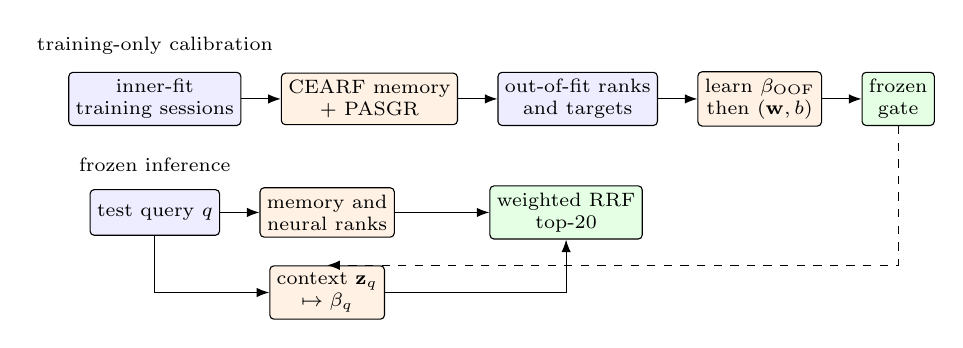
\begin{tikzpicture}[
  node distance=3.5mm and 5mm,
  box/.style={draw,rounded corners=1.5pt,align=center,
              minimum height=5.8mm,inner sep=2.5pt,font=\scriptsize},
  data/.style={box,fill=blue!7},
  model/.style={box,fill=orange!10},
  outputbox/.style={box,fill=green!10},
  arr/.style={-{Latex[length=1.6mm]},thin}
]
\node[data] (inner) {inner-fit\\training sessions};
\node[model,right=of inner] (experts) {CEARF memory\\+ PASGR};
\node[data,right=of experts] (oof) {out-of-fit ranks\\and targets};
\node[model,right=of oof] (learn) {learn $\beta_{\rm OOF}$\\then $(\mathbf w,b)$};
\node[outputbox,right=of learn] (freeze) {frozen\\gate};
\draw[arr] (inner)--(experts);
\draw[arr] (experts)--(oof);
\draw[arr] (oof)--(learn);
\draw[arr] (learn)--(freeze);

\node[data,below=8mm of inner] (query) {test query $q$};
\node[model,right=of query] (rank) {memory and\\neural ranks};
\node[outputbox,right=12mm of rank] (rrf) {weighted RRF\\top-20};
\node[model,below=3.5mm of rank] (beta) {
  context $\mathbf z_q$\\$\mapsto\beta_q$};
\draw[arr] (query)--(rank);
\draw[arr] (rank)--(rrf);
\draw[arr] (query) |- (beta);
\draw[arr] (beta) -| (rrf);
\draw[arr,dashed] (freeze.south) |- (beta.north);
\node[font=\scriptsize,above=1mm of inner] {training-only calibration};
\node[font=\scriptsize,above=1mm of query] {frozen inference};
\end{tikzpicture}
\caption{\method{} learns allocation from held-out \emph{training} sources,
freezes the gate, and then performs query-conditioned rank fusion.
Declared-validation/test labels never fit or select allocator parameters.}
\label{fig:method}
\end{figure}

\subsection{Leakage-safe training protocol}
Before modeling, a stable hash declares 5,000 validation queries; their
sources are ineligible for OOF calibration. A second hash removes at most
5,000 remaining training source sessions before expert fitting: 1,000 lock the
memory profile and 4,000 produce the ranks used in
Eqs.~\ref{eq:gate}--\ref{eq:loss}. Thus profile and gate subsets are disjoint,
and neither source session contributes events to the index or PASGR fit that
predicts its OOF target. Diginetica validation target events and incoming
transitions are removed from tuning histories. This is a single OOF holdout,
not full $K$-fold cross-fitting; allocator parameters remain frozen for final
test.

\section{Experimental Setup}
We derive 5-core leave-last-out histories from Amazon Reviews 2023 for Video
Games and Baby Products \cite{hou2024amazonreviews}; previously seen items are
masked. Diginetica uses its public session split and permits repeated items
\cite{diginetica2016}.
The domains contain respectively 25,613/36,014/43,098 items,
94,762/150,777/186,670 training sequences, and
94,762/150,777/60,858 test queries; 45\% of Diginetica queries but none of
the Amazon queries have $L\leq2$. We use ``sparse'' for item-frequency
sparsity: 27.9\%, 27.9\%, and 19.3\% of train-catalogue items occur at most
five times in Video, Baby, and Diginetica.
No sampled negatives are used at evaluation. We report Recall at 6, 10, and
20, nDCG at the same cutoffs, and
$U=.5\,\mathrm{R@6}+.5\,\mathrm{R@20}$; R@10 and all nDCG cutoffs guard
interpretation against that utility. Stochastic runs use seeds 42, 123, and
456. Main-table comparators are transition-only, V-SKNN, STAN, NARM, and a
SIGMA-compatible reimplementation; further baselines are
supplementary.

Allocation controls share identical expert ranks: equal mixing
($\beta=.5$), a learned OOF-global scalar, two independently learned
short/long scalars ($L\leq2$ versus longer; Amazon test rows use the longer
side), and Eq.~\ref{eq:gate}. We additionally test a
fixed deterministic reassignment of the frozen $\beta_q$ values across test
queries (preserving their exact multiset), a 16-unit MLP, the 16 target-free
diagnostics listed in the supplement, $k\in\{10,20,60\}$,
a min--max normalized CombSUM perturbation under frozen $\beta_q$ and
$\beta=.5$. The primary three-feature linear gate and $\Delta=.10$ are
fixed for all domains.

Paired per-query differences are averaged over matched seeds and bootstrapped
over query IDs with 20,000 repetitions. Intervals condition on three fitted
seeds; seed SD is reported separately. Experiments ran on an Apple M2 Pro with
32\,GB memory; CEARF uses one CPU process and PASGR uses Metal/MPS.

\section{Results}
\subsection{RQ1--RQ2: endpoints, baselines, and allocation}
% Generated by summarize_dynamic_beta.py; do not edit manually.
\begin{table}[t]
\caption{Compact allocation result on full-catalogue test queries. Values are matched-seed R@20 means. $\Delta U$ is dynamic minus OOF-global with a paired query-level 95\% bootstrap interval; complete cutoffs and seed SD are in the supplement.}
\label{tab:allocation-main}
\centering\scriptsize
\setlength{\tabcolsep}{2.7pt}
\resizebox{\textwidth}{!}{%
\begin{tabular}{lrrrrrrr}
\toprule
Domain & Memory & Neural & Equal $.5$ & OOF global & OOF short/long & Dynamic & $\Delta U$ [95\% CI]\\
\midrule
Video & .11901 & .12571 & .14610 & .14719 & .14726 & .14735 & +.00022 [+.00009,+.00035]\\
Baby & .03879 & .04873 & .05555 & .05671 & .05655 & .05669 & +.00002 [-.00003,+.00006]\\
Diginetica & .49428 & .44852 & .51430 & .51702 & .51692 & .51701 & +.00002 [-.00015,+.00018]\\
\bottomrule
\end{tabular}
}
\end{table}


\begin{table}[t]
\caption{Full-catalogue test R@20. \method{} uses \DynamicSeedCount{} seeds
and text teachers (cached teacher documented as E5-small on Video; TF--IDF/SVD
otherwise); comparator rows are ID-only, so this is system-level.
Transition/V-SKNN/STAN are deterministic; complete baselines and cutoffs are
supplementary. SIGMA-compatible is our reimplementation, not official SIGMA.}
\label{tab:baselines}
\centering\scriptsize
\setlength{\tabcolsep}{5pt}
\begin{tabular}{lrrr}
\toprule
Method & Video & Baby & Diginetica\\
\midrule
Transition-only & .04223 & .00735 & .40102\\
V-SKNN & .11936 & .05038 & .50506\\
STAN & .12115 & .04944 & .51502\\
NARM & .13705 & .02990 & \textbf{.53406}\\
SIGMA-compatible & .08644 & .02473 & .37219\\
\midrule
\method{} & \textbf{\DynamicVideoRtwenty} &
\textbf{\DynamicBabyRtwenty} & \DynamicDigiRtwenty\\
\bottomrule
\end{tabular}
\end{table}

Table~\ref{tab:allocation-main} first establishes complementarity. On every
domain, all fused allocations exceed both memory-only and neural-only at
R@20. Equal mixing already gives a large endpoint gain; thus most of the
improvement comes from heterogeneous evidence rather than gate complexity.
The fused system evaluated with dynamic allocation exceeds the stronger
endpoint by 17.2\% on Video, 16.3\% on
Baby, and 4.6\% on Diginetica.
The stricter comparison is against the training-only global and short/long
policies.

Table~\ref{tab:baselines} is system-level context, not a metadata-matched
architecture comparison. With the same cached teacher, NARM reaches
.15387/.06628 R@20 on Video/Baby, exceeding CEARF-N; hence Amazon claims are
allocation-orthogonal. Replacing PASGR by ID-only NARM inside the allocator
gives .14854/.05001/.53939 R@20 on Video/Baby/Diginetica, closing Diginetica
but losing Baby's metadata benefit. SIGMA-compatible underperforms
transition-only on Diginetica despite selected epochs 7/9/10, so it is only
context from our compatible reimplementation.

The final column of Table~\ref{tab:allocation-main} isolates the query-wise
correction. Dynamic allocation raises $U$ on Video Games with a paired
query-level interval above zero. It is not uniformly the best coarse-control
row in $U$: fixed $.5$, short/long, and head/tail are slightly higher on
Video, Baby, and Diginetica, respectively. Our claim is therefore narrower and
more falsifiable: a five-scalar, source-disjoint residual exposes query-level
expert advantage when it is stable while staying near the training-only global
prior when it is not. Baby has a much smaller positive mean shift whose interval
spans zero; Diginetica is likewise not detectably different from global. The gate can move
the global coefficient by at most .10. Video improves most at early ranks;
Baby's R@20 mean is slightly lower, so the correction is not uniform across
cutoffs.
On Video, dynamic-minus-global intervals are also above zero for R@6/R@10
(+.000278/+.000405) and nDCG@6/@10/@20
(+.000198/+.000238/+.000182), whereas R@20 is not; bounded correction changes
early ordering more clearly than broad top-20 coverage.

The fixed same-multiset reassignment control holds the distribution of
$\beta_q$ fixed while changing only query assignment. Relative to a fixed target-free
reassignment, the learned policy raises Video nDCG@20 by .000146
[.000082,.000210]; Diginetica has a supporting nDCG@10 difference of .000126
[.000033,.000221], while Baby intervals overlap zero. On Video, realized
neural-minus-memory nDCG@20 also changes from
\DynamicVideoLowBetaAdv{} in beta deciles 1--3 to
\DynamicVideoHighBetaAdv{} in deciles 8--10, a
\DynamicVideoAllocationGap{} separation. Its standardized length/frequency
coefficients are negative across all seeds and the tail coefficient is
nonnegative, assigning more neural mass to shorter, lower-frequency contexts.
Together, the fixed-reassignment and coefficient diagnostics are consistent
with heterogeneous expert-advantage regimes, beyond merely changing the
marginal weight distribution.

\subsection{RQ3: parsimony and sensitivity controls}
Capacity variants differ from the primary gate by only $O(10^{-4})$ in mean
$U$: the all-feature linear gate loses on one matched seed in each domain, and
Diginetica's best MLP is higher by only .00025. We keep the five-scalar form
instead of selecting a larger gate post hoc. Relaxing the residual bound also
does not explain the two null domains: $\Delta=.20$ gives the same Baby $U$
(.04343) and essentially the same Diginetica $U$ (.41329 versus .41332).

For each $k\in\{10,20,60\}$, the continuous prior and gate are refit on the
same OOF training ranks; no setting is selected on validation or test. The
primary $k=20$ has the highest mean $U$ on Video and Diginetica and lies
within $1.1\times10^{-4}$ of $k=60$ on Baby. Complete sensitivity and
fixed-allocation operator tables are in the supplement. Under frozen dynamic
allocation, weighted RRF exceeds normalized CombSUM in R@20 by
.00133/.00134/.00272 on Video/Baby/Diginetica; equal allocation reverses on
Diginetica, indicating operator--allocation compatibility rather than
unconditional RRF superiority.

\subsection{RQ4: inference cost}
For the timed seed-42 runs, the sum of separately measured warm medians
for feature construction and gate evaluation is
\DynamicRuntimeVideoGateUs{} $\mu$s/query
on Video, \DynamicRuntimeBabyGateUs{} on Baby, and
\DynamicRuntimeDigiGateUs{} on Diginetica. The jointly timed
feature+gate+RRF pipeline costs \DynamicRuntimeVideoPostUs{},
\DynamicRuntimeBabyPostUs{}, and
\DynamicRuntimeDigiPostUs{} $\mu$s/query, respectively. The supplement reports
the expert-inclusive cross-run estimate.
In a deterministic replay check, reconstructed $\beta_q$ values differ from
the original inference outputs by at most \DynamicRuntimeMaxBetaError{}, and
the top-20 rankings are reproduced exactly. Expert retrieval dominates latency; the
four-parameter residual gate is not the serving bottleneck.

\section{Conclusion and Limitations}
\method{} replaces validation-selected coarse mixing weights with a
source-disjoint query-invariant prior and a bounded query-wise residual law.
CEARF-N's main accuracy gain comes from expert complementarity; the residual
asks the harder, narrower question of whether any source-disjoint query signal
remains after a strong global prior. It does on Video's early ranks, while
Baby/Diginetica are reported as boundary cases. The five-scalar allocator is
cheap, bounded, score-scale invariant, and auditable.

Three domains do not establish universal transfer, and Diginetica lacks
original session IDs beyond expanded query rows for bootstrap clustering.
Only 41.7\%, 21.1\%, and 82.5\% of OOF calibration queries are actionable on
Video, Baby, and Diginetica; the allocator is therefore trained conditionally
on expert-union coverage, especially narrowly on Baby.
The PASGR cell was frozen by an upstream validation study;
our ``training-only'' claim applies specifically to allocation $\beta$, not
to every expert hyperparameter. Semantic metadata makes external comparisons
system-level; matched-teacher evidence exists only on Amazon. Finally, the
bounded query-wise residual gain over global fusion is small and undetectable
on two domains; larger untouched domains and temporal cross-fitting remain
necessary. Complete implementation details, allocation controls, and
statistical procedures are provided in the supplementary material.

\bibliographystyle{splncs04}
\bibliography{references_dynamic}
\end{document}
